\documentclass[11pt,english]{article}
\IfFileExists{lmodern.sty}{\usepackage{lmodern}}{}
\usepackage[T1]{fontenc}
\usepackage[latin9]{inputenc}
\usepackage{babel}
% Uncomment any of the following four lines to get different fonts
%\usepackage[garamondx,bigdelims]{newtxmath}
%\usepackage{garamondx}
%\usepackage{mathpazo}
%\usepackage{mathptmx}
\usepackage{newcent}

% Colors: see  http://www.math.umbc.edu/~rouben/beamer/quickstart-Z-H-25.html
\usepackage{color}
\usepackage[dvipsnames]{xcolor}
\definecolor{oucrimson}   {RGB}{132.,22. ,23. }
\definecolor{byublue}     {RGB}{0.  ,30. ,76. }
\definecolor{navyblue}    {RGB}{0.  ,0.  ,128.}
\definecolor{darkblue}    {RGB}{0.  ,0.  ,139.}
\definecolor{dukeblue}    {RGB}{0.  ,0.  ,156.}

% Layout
\usepackage{multirow}
\usepackage{setspace} %singlespacing; onehalfspacing; doublespacing; setstretch{1.1}
\setstretch{1.5}
\usepackage[verbose,margin=1in]{geometry} % Margins
\setlength{\headheight}{15pt} % Sufficent room for headers
\usepackage[bottom]{footmisc} % Forces footnotes on bottom

%-- coding: UTF-8 --
\usepackage[UTF8]{ctex}

% Headers/Footers
\usepackage{lastpage}
\setlength{\headheight}{0pt}
\usepackage{fancyhdr}
\pagestyle{fancy}
\fancyhf{}\renewcommand{\headrulewidth}{0pt}
\lhead{} \chead{} \rhead{}

\rfoot{Page \thepage \,of 3}

% Useful Packages
%\usepackage{bookmark} % For speedier bookmarks
%\usepackage{amsthm}   % For detailed theorems
%\usepackage{amssymb}  % For fancy math symbols
%\usepackage{amsmath}  % For awesome equations/equation arrays
\usepackage{array}    % For tubular tables
\usepackage{booktabs}
\usepackage{longtable}% For long tables
\usepackage[flushleft]{threeparttable} % For three-part tables
\usepackage{multicol} % For multi-column cells
\usepackage{graphicx} % For shiny pictures
\usepackage{subfig}   % For sub-shiny pictures
\usepackage{enumerate}% For cusomtizable lists
%\usepackage{pstricks,pst-node,pst-tree,pst-plot} % For trees

% Bib
\usepackage[authoryear]{natbib} % Bibliography
\usepackage{url}                % Allows urls in bib
\usepackage{indentfirst}
% TOC
\setcounter{tocdepth}{4}

% Links
\usepackage{hyperref}    % Always add hyperref (almost) last
\hypersetup{colorlinks,breaklinks,citecolor=black,filecolor=black,linkcolor=oucrimson,urlcolor=oucrimson}
\usepackage[all]{hypcap} % Links point to top of image, builds on hyperref
\usepackage{breakurl}    % Allows urls to wrap, including hyperref

% Custom commands
\newcommand{\makeheading}[2]%
        {\hspace*{-\marginparsep minus \marginparwidth}%
         \begin{minipage}[t]{\textwidth\marginparwidth\marginparsep}%
         {\LARGE\bfseries #1} \hfill  {\LARGE\bfseries #2 \hspace*{-2.3\marginparsep minus \marginparwidth}}\\[-0.2\baselineskip]%
                 \rule{\textwidth}{1.5pt}\rule{\marginparsep}{1.5pt}\rule{\marginparwidth}{1.5pt}%
         \end{minipage}}

\setlength{\parindent}{0in}
\reversemarginpar
\renewcommand{\section}[2]{
        \pagebreak[3]%
        \vspace{1.0\baselineskip}%
        \phantomsection\addcontentsline{toc}{section}{#1}%
        \hspace{0in}%
        %\marginpar{\raggedright \scshape #1}#2}
        %\rule[3.5pt]{0.9in}{1.5pt} ~~
        {\raggedright \scshape \large \textbf{#1}}%
        \vspace{0.25\baselineskip}#2
}


\begin{document}
%\thispagestyle{empty}
\makeheading{Jiahe Li}{Curriculum Vitae}


% ADDRESS/CONTACT HEADER
% ==================================================================================
\setstretch{1.0}
\begin{multicols}{2}

\begin{flushleft}
Junior in Computer Engineering

ZJU-UIUC institute

No.718, Haizhou East Road

Haining, Zhejiang, China


~\       


\textit{Phone:} +86 15069025932

\textit{E-mail:} \href{jiahe.20@intl.zju.edu.cn}{jiahe.20@intl.zju.edu.cn}

\textit{Homepage:} \href{erikaqvq.github.io}{https://erikaqvq.github.io}


\end{flushleft}



% ==================================================================================




\begin{flushright}
   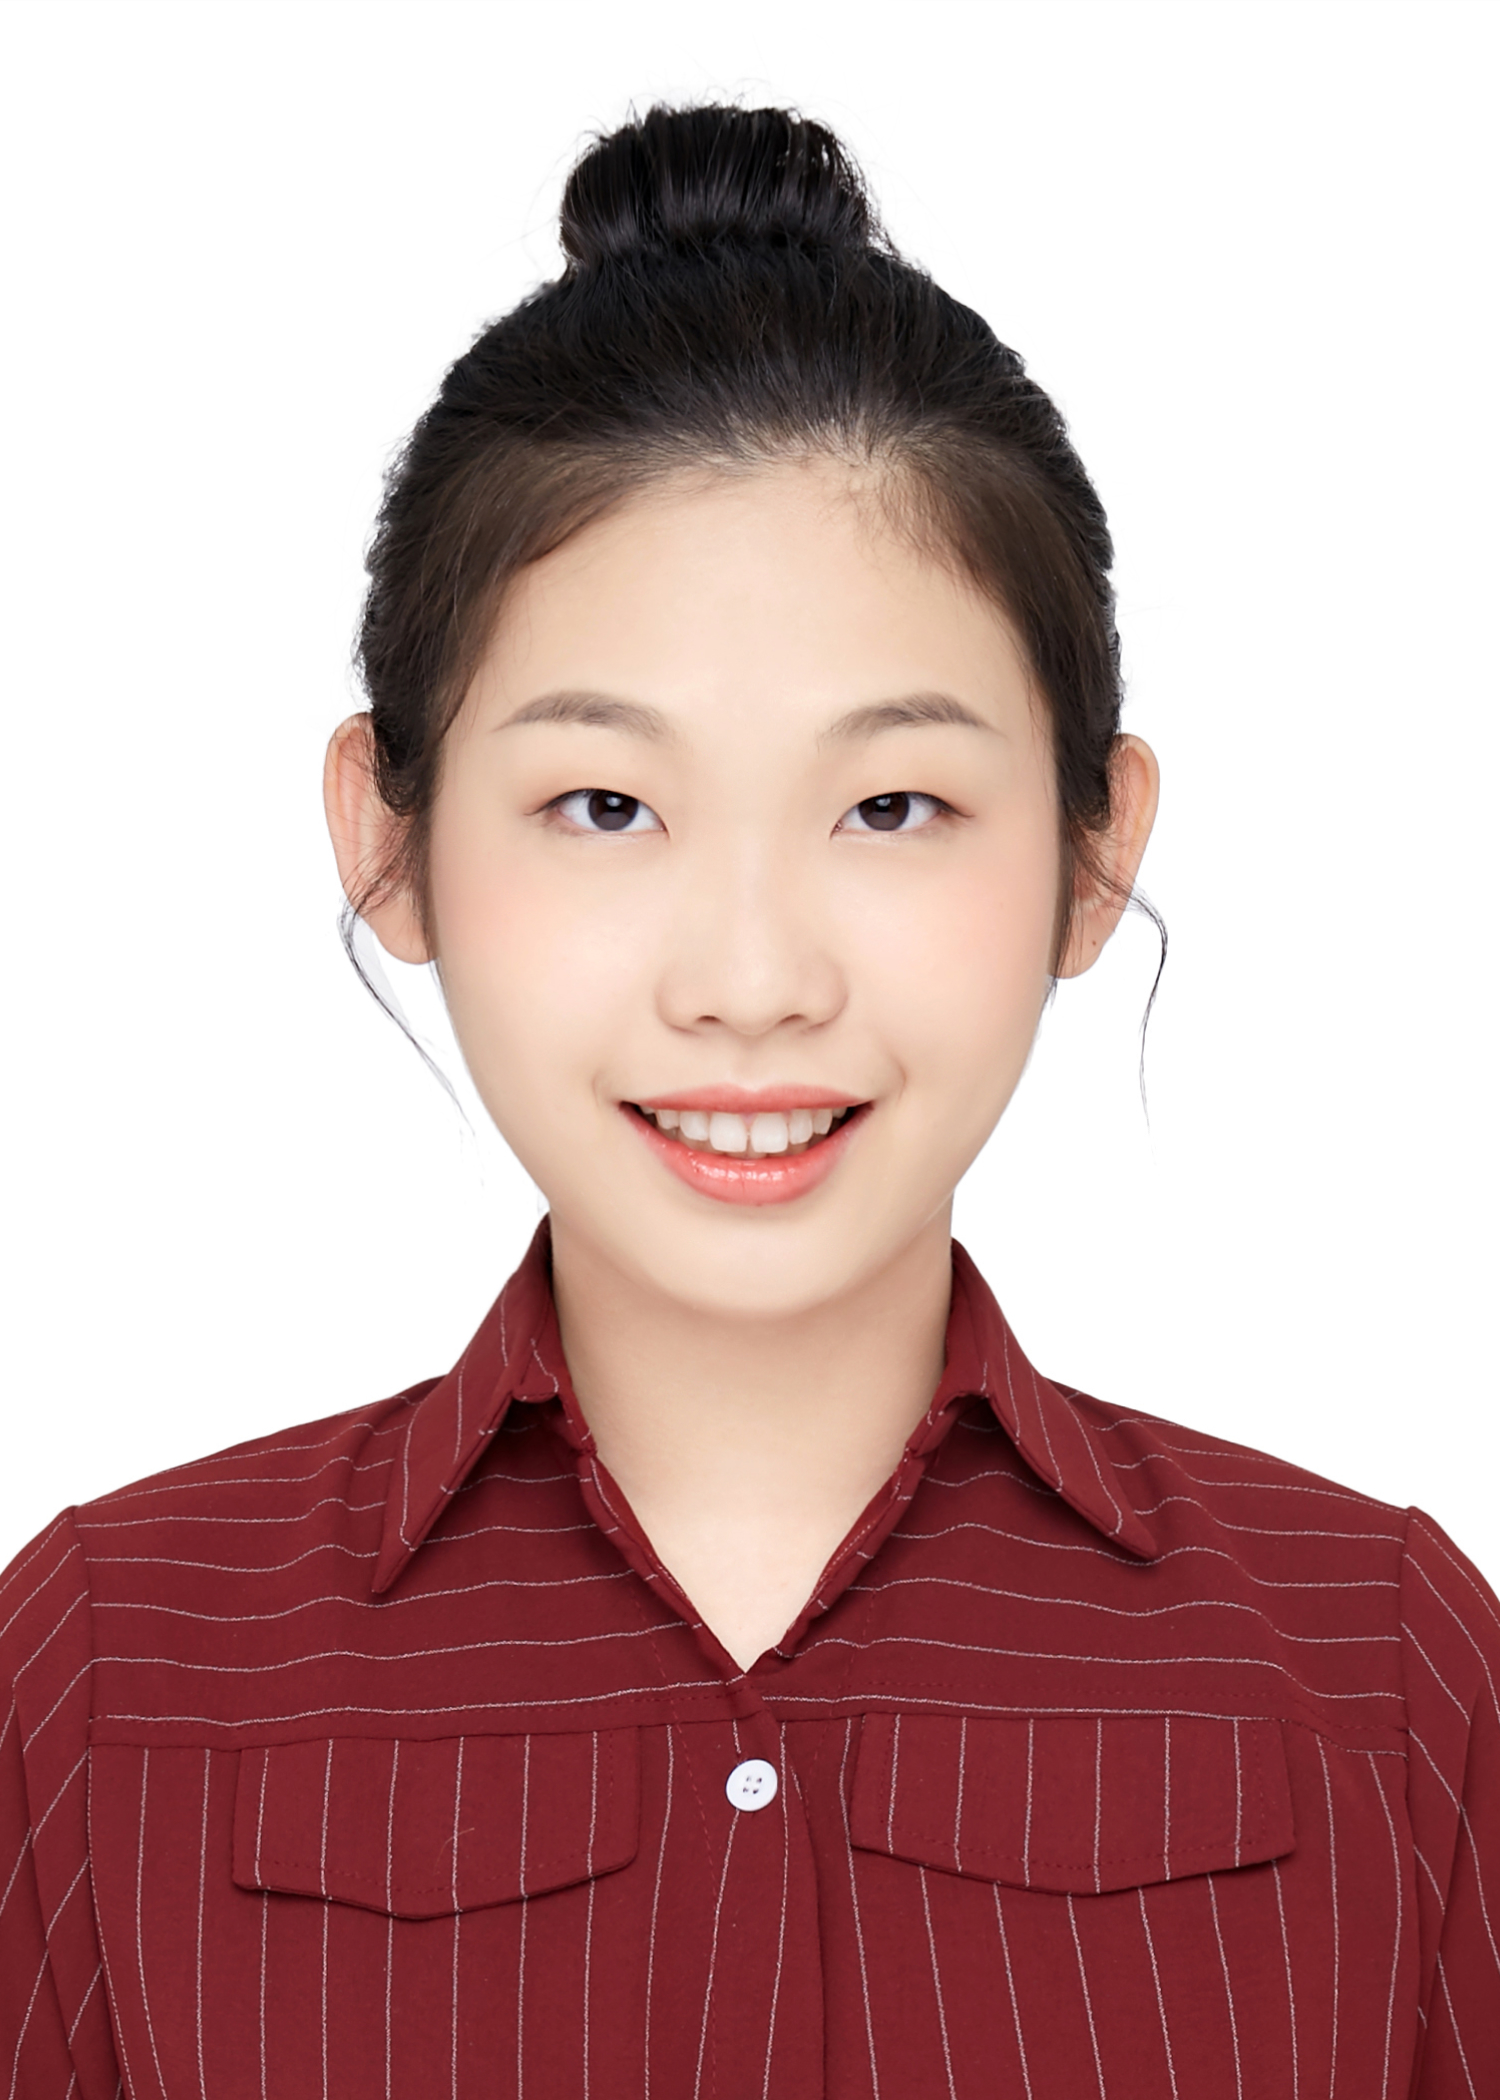
\includegraphics[scale=0.3]{img.jpg} 
\end{flushright}
\end{multicols}
\setstretch{1.2}
\vspace{-.25in}
\section{Education}\\
% ==================================================================================
\begin{tabular}{p{1.5in}>{\hangindent=1em}p{5.05in}<{\raggedright}}
2022.8 - 2022.12 & Exchange(CompE) at UIUC \\ 
2020.9 - Present & B.A. in CompE, ZJUI \\
2017.9 - 2020.6 & Shandong Experimental High School (Senior High) \\
\end{tabular}

~\\

 \qquad I started learning programming and algorithms in high school. After a year of study, I achieved the first prize in Shandong Province in the National Junior Informatics Olympiad NOIP2018. The experience of studying informatics competitions has given me strong independent learning ability and I have developed a stronger interest in the computer engineering.
 
~\

 \qquad In the past six semesters in ZJU-UIUC institute, I have earned 135 credits with a cumulative GPA of \textbf{3.95}, ranking \textbf{TOP 1} in my major. In the fall semester of 2022, I went to UIUC as an exchange student.

 ~\

\section{Major Awards}\\
% ==================================================================================
\begin{tabular}{p{1.5in}>{\hangindent=1em}p{5.05in}<{\raggedright}}
2021 & \textbf{National Scholarship of China} \\
2022 & Zhejiang Provincial Government Scholarship \\
2022 & The Mathematical Contest in Modeling - Honorable Mention \\
2022 & Outstanding student association leaders of Zhejiang University \\
2022 & Dean's List of ZJU-UIUC Institute  \\
2021 & Outstanding student association leaders of Zhejiang University \\
2021 & Dean's List of ZJU-UIUC Institute  \\
2018 & National Olympiad in Informatics in Provinces (NOIp) - First Prize \\

\end{tabular}

\pagebreak{}

\section{Publications}\\
Haoran Deng, Yang Yang, \textbf{Jiahe Li}, Haoyang Cai, Shiliang Pu, and Weihao Jiang. Accelerating Dynamic Network Embedding with Billions of Parameter Updates to Milliseconds. In Proceedings of the Twenty-Ninth ACM SIGKDD International Conference on Knowledge Discovery and Data Mining (KDD'23), 2023.

\section{Research Experience}\\
% ==================================================================================
\vspace{-1mm}
\begin{tabular}{p{1.5in}>{\hangindent=1em}p{5.05in}<{\raggedright}}
\textbf{2023.1 - Now} & \textbf{Dynamic Network Embedding at AINet Lab, ZJU}\\
  & Advisor: Prof. Yang Yang, ZJU\\
\end{tabular}

~\

\qquad Network embedding, a graph representation learning method illustrating network topology by mapping nodes into lower-dimension vectors, is challenging to accommodate the ever-changing dynamic graphs in practice. We propose the Dynamic Adjacency Matrix Factorization (DAMF) algorithm, which achieves an efficient and accurate dynamic network embedding by rotating and scaling the coordinate system where the network embedding resides with no more than the number of edge modifications changes of node embeddings. Moreover, a dynamic Personalized PageRank is applied to the obtained network embeddings to enhance node embeddings and capture higher-order neighbor information dynamically. We unprecedentedly expand dynamic network embedding experiments to billion-edge graphs, where DAMF updates billion-level parameters in less than 10ms.

~\

\vspace{-1mm}
\begin{tabular}{p{1.5in}>{\hangindent=1em}p{5.05in}<{\raggedright}}
\textbf{2022.6 - 2022.8} & \textbf{Container Vulnerability Reachability at NESA Lab, ZJU}\\
  & Advisor: Prof. Xuhong Zhang and Shouling Ji, ZJU\\
\end{tabular}

~\

\qquad Bloated dependencies are libraries that are packed with the compiled code of an application but are not required to create and run the application. DepClean is a way to automatically clean up a Java project's dependency tree and remove dependencies that are not necessary for building the project. My team members and I learned about this method during our summer research and proposed an optimization that shrinks the unit of dependency study from a file to a function.

~\

\begin{tabular}{p{1.5in}>{\hangindent=1em}p{5.05in}<{\raggedright}}
\textbf{2021.6 - 2022.3}   & \textbf{Path ORAM (Cryptography) at ABC Lab, ZJU}\\
  & Advisor: Prof. Jian Liu, ZJU\\
\end{tabular}

~\

\qquad Oblivious RAM hides the memory access pattern by using extra bandwidth and memory overhead. Path ORAM stores memory blocks on a binary tree's random branch. Because the blocks are positioned on distinct branches, repeated procedures reveal no information. rORAM is an optimization of Path ORAM to achieve faster interval queries by saving multiple binary trees. Another spatial optimization of Path ORAM is to use B-tree instead of linear position map storage. After studying, I found that by combining the two optimizations, I can take full advantage of both and make progress in both time and space.

~\


\section{Extracurricular activities}\\
% % ==================================================================================
\begin{tabular}{p{1.5in}>{\hangindent=1em}p{5.05in}<{\raggedright}}
\textbf{2020.9 - 2022.9} & \textbf{President of Room78 Algorithm Club, Zhejiang University} \\
\end{tabular}

~\

 \qquad In my freshman year, I, as the founder, led like-minded students to create the Room78 Algorithm Club. I worked as the \textbf{president of Room78} during my 1st and 2nd years and conducted many algorithm discussions and activities. The club was awarded as the outstanding club in 2021. I was awarded as the outstanding club leader in 2021, 2022.

~\ 

\begin{tabular}{p{1.5in}>{\hangindent=1em}p{5.05in}<{\raggedright}}
\textbf{2021.7 - 2022.2} & \textbf{Security Consultant of 
Hepta Workshop, ZJU-UIUC Institute}  \\
\end{tabular}

~\

\qquad I have been one of the security consultants for Hepta Workshop since 2021, contributing the security foundation in \href{https://github.com/HeptaDevGrp/EmailServer}{Email Server} build.

~\

\begin{tabular}{p{1.5in}>{\hangindent=1em}p{5.05in}<{\raggedright}}

\textbf{2015.4 - Present} & \textbf{Museum Docent at Shandong Museum} \\
\end{tabular}

~\

  \qquad In 2015, I joined the Shandong Museum Volunteer Docent Team. I have accumulated more than 300 hours of volunteer service. After leaving my hometown for college, I still use my summer and winter time for volunteer work.

%\pagebreak{}

\section{Course Projects}\\ %\vspace{-7.5mm}
% ==================================================================================
\begin{tabular}{p{1.5in}>{\hangindent=1em}p{5.05in}<{\raggedright}}
\textbf{2022.9 - 2022.12} & \textbf{\href{https://github.com/Erikaqvq/MongOS}{MongOS}, Operating System Design, ECE391} \\
\end{tabular}

~\

\qquad Based on the foundation provided by the course, we designed a Linux-like operating system, implementing virtual memory (paging and segmentation), file system, interrupt handlers, system call handlers, exception handlers, multi-terminal, scheduler, etc.

~\

\begin{tabular}{p{1.5in}>{\hangindent=1em}p{5.05in}<{\raggedright}}
\textbf{2022.9 - 2022.12} & \textbf{\href{https://github.com/Erikaqvq/DailylifeXcov19}{DailylifeXcov19}, Database Design, CS411} \\
\end{tabular}

~\

\qquad Daily life with COVID-19 is a comprehensive database of COVID-19 information. The first functionality is COVID-19 basic data, such as the number of confirmed diagnoses, cures, deaths, and vaccinations in each country. The second is COVID-19-related news and rumors, as well as social media discussions about it.

~\

\begin{tabular}{p{1.5in}>{\hangindent=1em}p{5.05in}<{\raggedright}}
\textbf{2022.3 - 2022.6} & \textbf{\href{https://github.com/Erikaqvq/MeT-System}{MeT-System}, Reservation and Queuing System Design, CS225} \\
\end{tabular}

~\

\qquad MeT System is an integrated medical system for medical treatment that allows for registration, queuing, scheduling of treatment, printing of reports, etc. In this system, users have a high degree of freedom to receive treatment or not, and will be scheduled fairly and efficiently. The core data structures are Fibonacci heap and B+ tree.

\end{document}

%%%%%%%%%%%%%%%%%%%%%%%%%% End CV Document %%%%%%%%%%%%%%%%%%%%%%%%%%%%%
